\let\negmedspace\undefined
\let\negthickspace\undefined
\documentclass[journal]{IEEEtran}
\usepackage[a5paper, margin=10mm, onecolumn]{geometry}
\usepackage{lmodern} % Ensure lmodern is loaded for pdflatex
\usepackage{tfrupee} % Include tfrupee package

\setlength{\headheight}{1cm} % Set the height of the header box
\setlength{\headsep}{0mm}     % Set the distance between the header box and the top of the text

\usepackage{gvv-book}
\usepackage{gvv}
\usepackage{cite}
\usepackage{amsmath,amssymb,amsfonts,amsthm}
\usepackage{algorithmic}
\usepackage{graphicx}
\usepackage{textcomp}
\usepackage{xcolor}
\usepackage{txfonts}
\usepackage{listings}
\usepackage{mathtools}
\usepackage{gensymb}
\usepackage{enumitem}
\usepackage{comment}
\usepackage[breaklinks=true]{hyperref}
\usepackage{tkz-euclide} 
\usepackage{listings}
\usepackage{gvv}                                        
\def\inputGnumericTable{}                                 
\usepackage[latin1]{inputenc}                                
\usepackage{color}                                            
\usepackage{array}                                            
\usepackage{longtable}                                       
\usepackage{calc}                                             
\usepackage{multirow}                                         
\usepackage{hhline}                                           
\usepackage{ifthen}                                           
\usepackage{lscape}
\begin{document}

\bibliographystyle{IEEEtran}
\vspace{3cm}

\title{9.9.5.10}
\author{EE24BTECH11010 - Balaji B}
% \maketitle
% \newpage
% \bigskip
{\let\newpage\relax\maketitle}
\textbf{Question:}\\
Find the area of the region included between the circle $x^2 + y^2 = 8x$ and inside of the parabola $y^2 = 4x$. \\
\textbf{Answer:}
\begin{table}[h!]
    \centering
    \begin{tabular}[12pt]{ |c| c| c|c|c|c|}
    \hline
    $X$ & 1 & 2 & 3 & 4 & 5 \\
    \hline
    $P(X)$ & $K$ & 2$K$ & 2$K$ & 3$K$ & $K$ \\
    \hline 
    \end{tabular} 

    \caption{Variables used}
    \label{tab1-1.2-20}
\end{table} 

The conic parameter for the circle and parabola  can be expressed as 
\begin{align}
    \vec{V}_1 = \myvec{1 & 0 \\ 0 & 1}, \vec{u}_1 = \myvec{-4 \\ 0}, f_1 = 0 \\
    \vec{V}_2 = \myvec{0 & 0 \\ 0 &1}, \vec{u}_2 = \myvec{-2 \\ 0}, f_2 = 0
\end{align}
Substituting the values of $\vec{V_i}$, $\vec{u_i}$, $f_i$, $i = 1, 2$, for pair of straight lines\\
\begin{align}
 \mydet{\vec{V}_1 + \mu\vec{V}_2 & \vec{u}_1 + \mu\vec{u}_2 \\ (\vec{u}_1+ \mu\vec{u}_2)^\top & f_1 + \mu f_2} = 0 \\
 \mydet{1 & 0 & -4 -2\mu \\ 0 & \mu + 1 & 0 \\ -4-2\mu & 0 & 0} = 0   \\
 \mu = -1
\end{align}
The equation of the pair of straight line, is given by
\begin{align}
    \vec{x}^\top (\vec{V}_1+\mu\vec{V}_2)\vec{x}+2(\vec{u}_1 + \mu \vec{u}_2)^\top \vec{x} + (f_1 + \mu f_2) &= 0 \\
    \vec{x}^\top \myvec{1 & 0 \\ 0 & 0}\vec{x}+2\myvec{-2 & 0} \vec{x}   = 0  \\
    \sbrak{\vec{x}^\top \myvec{1 & 0 \\ 0 & 0} + \myvec{-4 & 0}}\vec{x} = 0
\end{align}
$\because \vec{x} = \myvec{x \\ y}$, substituting it we get
\begin{align}
    \sbrak{\myvec{x & y}\myvec{1 & 0 \\ 0 & 0} + \myvec{-4 & 0}}\myvec{x \\ y} \\
    \myvec{x-4 & 0}\myvec{x \\ y } = 0 \\
    (x -4)(x) = 0 \\
    \therefore x = 0, x = 4
\end{align}
The equation of the lines are
\begin{align}
    \vec{x} = \myvec{0 \\ 0} + \kappa\myvec{0 \\ 1} \text{ and }
    \vec{x} = \myvec{4 \\ 0} + \kappa\myvec{0 \\ 1}
\end{align}
$\therefore $The intersection of Circle and Parabola is lines with parameters
\begin{align}
\vec{m}_1 = \myvec{0 \\ 1}, \vec{h}_1 = \myvec{0 \\ 0} \\
\vec{m}_2 = \myvec{0 \\ 1}, \vec{h}_2 = \myvec{4 \\ 0}
\end{align}
Substituting the line-1 equation in parabola equation gives the value of $\kappa$
\begin{align}
\brak{\vec{h}+\kappa\vec{m}}^\top\vec{V}\brak{\vec{h}+\kappa\vec{m}} + 2\vec{u}^\top\brak{\vec{h}+\kappa\vec{m}} + f &= 0 \\
\brak{\myvec{0 \\ 0} + \kappa \myvec{0\\1}}^\top \myvec{ 0&0\\0&1}\brak{\myvec{0 \\ 0}+ \kappa \myvec{0\\1}} + 2\myvec{-2\\0}^\top \brak{\myvec{0 \\ 0} + \kappa \myvec{0\\1}} + 0 = 0 \\
\myvec{0 & \kappa}\myvec{0 & 0 \\ 0 &1}\myvec{0 \\ \kappa} + 2\myvec{-2 & 0}\myvec{0 \\ \kappa} = 0
\end{align}
\begin{align}
    \kappa^2 = 0 \\
    \kappa_1 = 0
\end{align}
The intersection point of line-1 with parabola
\begin{align}
    \vec{x}_1 &= \vec{h}_1 + \kappa_1\vec{m}\\
    \vec{x}_1 &= \myvec{0 \\ 0}
\end{align}
Substituting the line-2 equation in parabola equation gives the value of k
\begin{align}
    \brak{\myvec{4\\0}+\kappa\myvec{0\\1}}^\top\myvec{0 & 0\\0 & 1}\brak{\myvec{4\\0}+\kappa\myvec{0\\1}} + 2\myvec{-2\\0}^\top\brak{\myvec{4\\0}+\kappa\myvec{0\\1}} + 0 &= 0\\
\myvec{4&\kappa}\myvec{0&0\\0&1}\myvec{4\\\kappa}+2\myvec{-2&0}\myvec{4\\\kappa} &= 0\\
\kappa^2 - 16 = 0 \\
\kappa_1 = 4 \\
\kappa_2 = -4
\end{align}
The intersection points of line-2 with parabola 
\begin{align}
\vec{x_2} &= \myvec{4\\4}\\
\vec{x_3} &= \myvec{4\\-4}
\end{align}
The desired area is given by 
\begin{align}
    A &= 2\sbrak{\int_{0}^{4}\sqrt{4x}dx + \int_{4}^{8}\sqrt{8x - x^2} } \\
    A &= 2\sbrak{\sbrak{\frac{4}{3} x^{\frac{3}{2}}}_{0}^{4} + \sbrak{\frac{x-4}{2}\sqrt{8x - x^2} + 8 \sin^{-1}\brak{\frac{x-4}{4}}}_4^8 }\\
     A &= \frac{64}{3}+ 8 \pi
\end{align}
$\therefore$ The Area $A$ is $\frac{64}{3} + 8\pi$
\begin{figure}[h!]
   \centering
   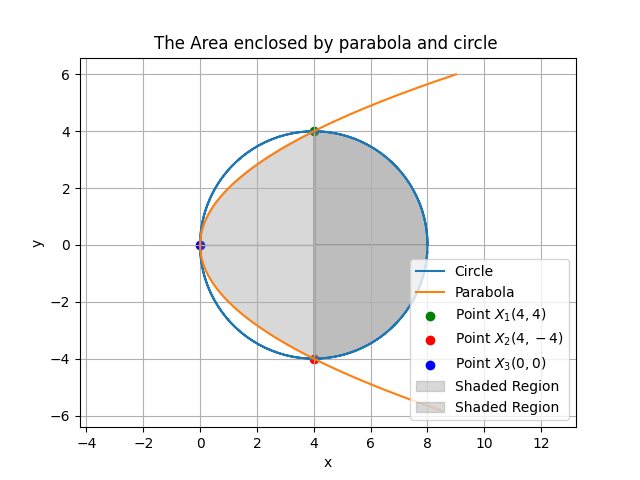
\includegraphics[width = .7\linewidth]{figs/fig.png}
   \caption{The Area enclosed by parabola and circle}
   \label{stemplot}
   \end{figure}

\end{document}
